% CVPR 2024 Paper Template; see https://github.com/cvpr-org/author-kit

\documentclass[10pt,twocolumn,letterpaper]{article}

%%%%%%%%% PAPER TYPE  - PLEASE UPDATE FOR FINAL VERSION
% \usepackage{cvpr}              % To produce the CAMERA-READY version
\usepackage[review]{cvpr}      % To produce the REVIEW version
% \usepackage[pagenumbers]{cvpr} % To force page numbers, e.g. for an arXiv version

% Import additional packages in the preamble file, before hyperref
\input{preamble}

% It is strongly recommended to use hyperref, especially for the review version.
% hyperref with option pagebackref eases the reviewers' job.
% Please disable hyperref *only* if you encounter grave issues, 
% e.g. with the file validation for the camera-ready version.
%
% If you comment hyperref and then uncomment it, you should delete *.aux before re-running LaTeX.
% (Or just hit 'q' on the first LaTeX run, let it finish, and you should be clear).
\definecolor{cvprblue}{rgb}{0.21,0.49,0.74}
\usepackage[pagebackref,breaklinks,colorlinks,citecolor=cvprblue]{hyperref}

%%%%%%%%% PAPER ID  - PLEASE UPDATE
\def\paperID{1} % *** Enter the Paper ID here
\def\confName{Computer Vision}
\def\confYear{2024}

%%%%%%%%% TITLE - PLEASE UPDATE
\title{\LaTeX\ Proposal for \confName~}
%%%%%%%%% AUTHORS - PLEASE UPDATE
\author{Murtadha Marzouq\\
{\tt\small Graduate Student}\\
{\tt\small mmarzouq@charlotte.edu}
% For a paper whose authors are all at the same institution,
% omit the following lines up until the closing ``}''.
% Additional authors and addresses can be added with ``\and'',
% just like the second author.
% To save space, use either the email address or home page, not both
\and
Param Patel\\
{\tt\small Graduate Student}\\
{\tt\small ppate211@charlotte.edu}
\and 
Haochen Ye\\
{\tt\small Graduate Student}\\
{\tt\small \small hye5@charlotte.edu}
\and
Sam Aldehayyat\\
{\tt\small Undergraduate Student}\\
{\tt\small saldehay@charlotte.edu}
\and
Yuepei Yu\\
{\tt\small Undergraduate Student}\\
{\tt\small yyu20@uncc.edu}
}



\toggletrue{cvprfinal} % REVIEW VERSION


\begin{document}
\maketitle
\begin{abstract}

Sam This Computer Vision project proposal will contain problem statement and importance, plan for data sources, and the computer vision algorithm to be used in this project.
\end{abstract}
    
\section{Introduction}
\label{sec:intro}

Attendance is an indispensable metric for a student's academic journey, where consistent participation correlates with academic success. The process of monitoring and maintaining attendance records presents significant challenges, which mostly originates from constraints in time and resources. By harnessing the benefits of computer vision, this project addresses the problem of automating the attendance-taking process in classrooms using a tool that is at every teacher’s disposal, their cell phone camera.

\section{Problem Statement}
\label{sec:problem}
Attendance enforcement and record keeping in the class room is often overlooked because of added time and resources. Additionally, the COVID-19 pandemic has made it difficult to enforce attendance in the classroom. In this project, we will develop a system that will allow students to check in and out of a classroom using facial recognition. The system will be able to identify the student and record the time they entered and exited the classroom. The system will also be able to identify the number of students in an image and cross-reference it with Canvas's people table (number of students) to provide a percentage of students in the classroom.
%-------------------------------------------------------------------------

\section{Data}
1. The data for this project will be collected from the University of North Carolina's Canvas API (Will use Murtadha's Account) to fetch the number of students in the Computer Vision course. This information will be stored to be references to give a percentage of students attending.\\
2. The dataset that will be used to train our model is the \href{http://vis-www.cs.umass.edu/lfw/}{\underline{Faces in the Wild (LFW)}} dataset. This dataset contains more than 13,000 images of faces collected from the web. Each face has been labeled with the name of the person pictured. 1680 of the people pictured have two or more distinct photos in the dataset. The only constraint on these faces is that they were detected by the Viola{-}Jones face detector.\\
3. Images of the students in the class will be collected using a webcam. The images will be taken in the classroom and will be used to train the model to recognize the students in the class.\\
\input{sec/3_data_analysis}
\section{Methodology \& Computer Vision Algorithm}
\label{sec:method}
\subsection{Methodology}
\label{subsec:method}
1. Research datasets to use \cite{YOLOpaper2}
2. Research models to use 
3. Selected COCO Dataset and YOLOv6 \cite{YOLOpaper1} model
4. Train that model to recognize humans in an image\\
5. Test the trained model to recognize the students in the class from images taken by group members\\

The model will be trained using a portion of the Microsoft COCO dataset. The model will be used to recognize the students in the class, apply bounding boxes around the students recognized and sum up the number of bounding boxes to get a total count of students in that image. As an addition, we noticed that we were not able to capture an entire classroom in 1 image from the front, we have also presented an option to the instructor to take numerous pictures and stitch them together into 1 image and then do a total sum of students found.\\ 

\subsection{Computer Vision Algorithm}
\label{subsec:Computer Vision Algorithm - YOLOv6}
We chose to use the YOLO (You Only Look Once) \cite{YOLO} model. YOLO uses a single neural network to simultaneously predict bounding boxes and class probabilities, making it ideal for applications demanding instantaneous detection such as our project. \\
Since it's introduction in 2016, YOLO has undergone significant improvements. YOLOv2 was released in 2017, YOLOv3 in 2018, etc. these numerous iteration included refined accuracy and speed, and incorporated multiple scales for object detection. YOLO showcases the hallmarks of a good model due to it's advancements that continue to propel it to the forefront of real-time object detection technology. This lengthy history also makes it an ideal choice to use for our project since we can easily find numerous resources and blog posts referring this model.\\
% Diagram of the system%
\begin{figure}[h]
    \centering
    \includegraphics[width=0.5\textwidth]{images/Diagram-1.png}
    \caption{Flowchart of the system}
    \label{fig:flowchart}
\end{figure}

%-------------------------------------------------------------------------

\graphicspath{ {images} }

\section{Team}
    \includegraphics[width=0.1\textwidth]{Murtadha.jpg}\\ \textbf{Murtadha Marzouq}\\ \href{https://webpages.charlotte.edu/mmarzouq/English/Resume.pdf}{\underline{Resume Link}}\\
   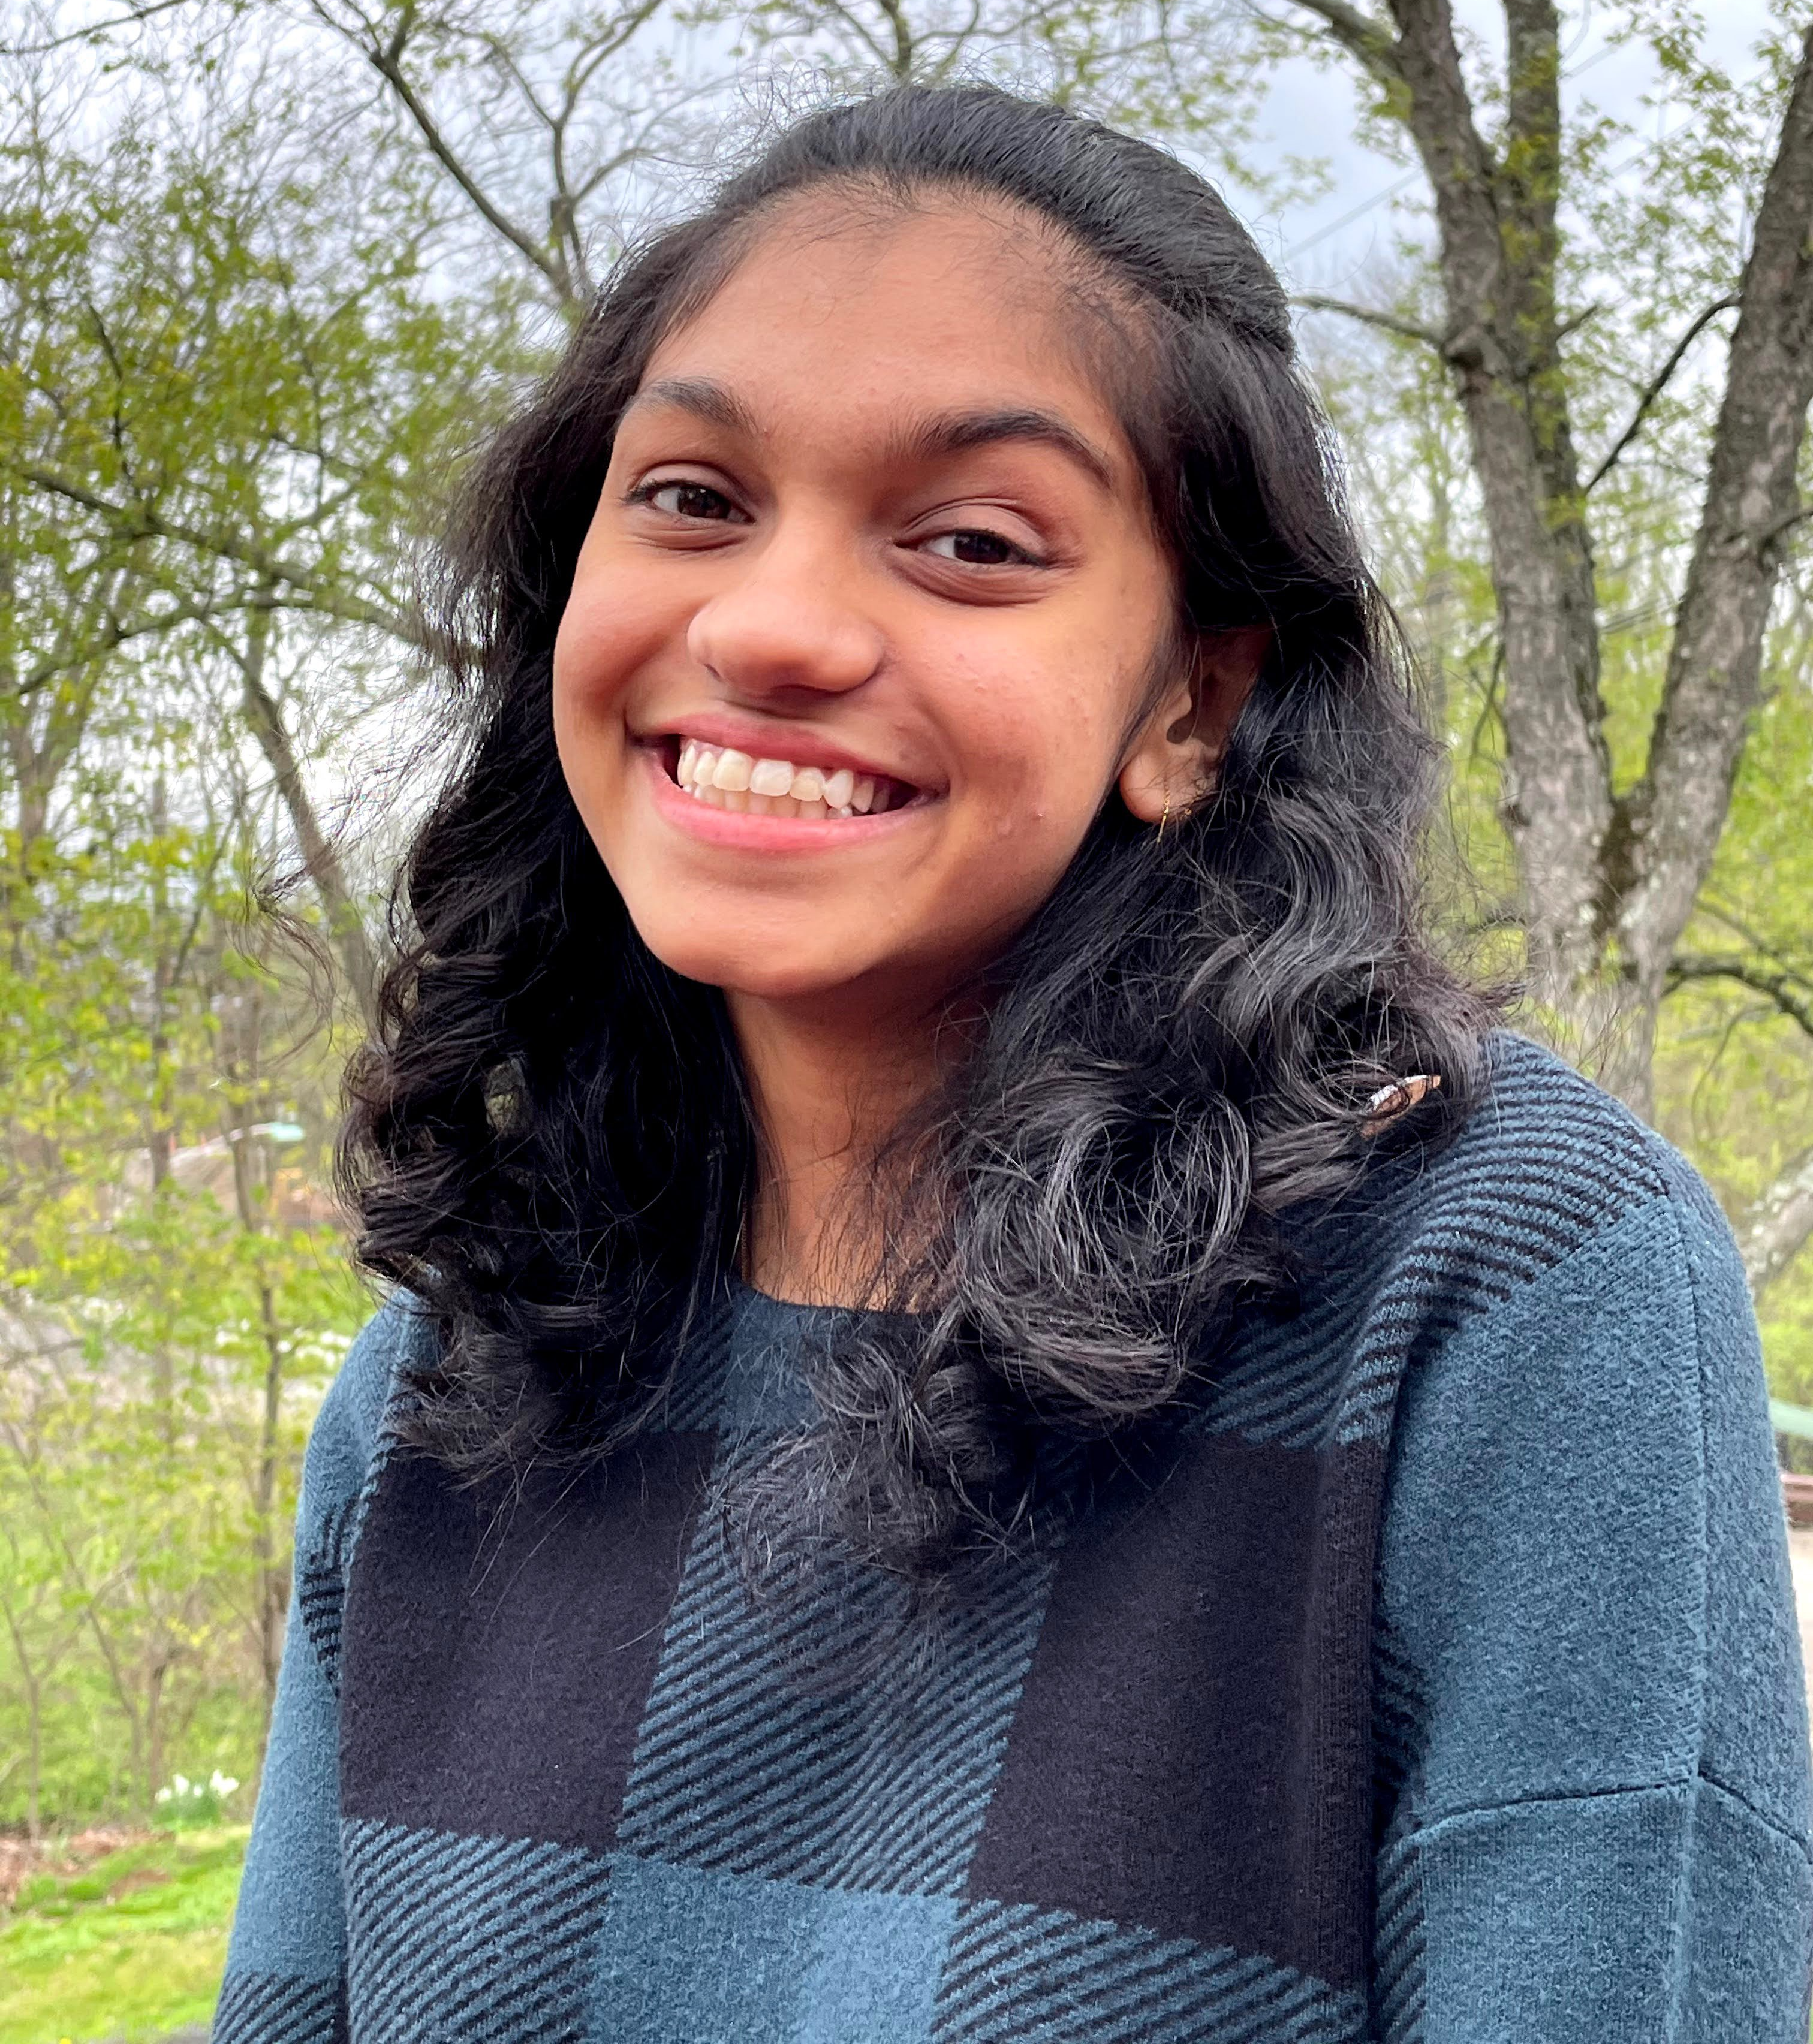
\includegraphics[width=0.1\textwidth]{Param.png}\\ \textbf{Param Patel}\\  \href{https://drive.google.com/file/d/13jr45PMGy9iJG0CavpYmuiN5SDwGgygj/view?usp=sharing}{\underline{Resume Link}}\\
\includegraphics[width=0.1\textwidth]{Haochen.png}\\     \textbf{Haochen Ye}\\ \href{https://drive.google.com/file/d/1YOZvJANmngCAai1OxXm28a_7XmKGmpH1/view?usp=sharing}{\underline{Resume Link}}\\
\includegraphics[width=0.1\textwidth]{Sam.png}\\     \textbf{Sam Aldehayyat}\\ \href{https://drive.google.com/file/d/14jBT5AZ_GzdElLh-0LSXzP7AxgjMu0wa/view?usp=sharing}{\underline{Resume Link}}\\
\includegraphics[width=0.1\textwidth]{Yuepei.png}\\     \textbf{Yuepei Yu}\\ \href{https://drive.google.com/file/d/1xcBhl6kxY1gQZsCjADVlJvvDVYBJLoSo/view?usp=sharing}{\underline{Resume Link}}\\
This team had been build with the following fellowship in minds:\\
1. Liberté, Egalité, Fraternité\\
2. Diversity and Inclusion\\
3. Teamwork\\
4. Respect\\
5. Integrity\\


{
    \small
    \bibliographystyle{ieeenat_fullname}
    \bibliography{main}
}
% WARNING: do not forget to delete the supplementary pages from your submission 
% \input{sec/X_suppl}

\end{document}

